\section{第七章}

\subsection{题目1}

已知观测数据
\begin{table}[H]
\centering
\begin{tabular}{llllll}\hline
x    & -2 & -1 & 0 & 1 & 2 \\ \hline
f(x) & 0  & 1  & 2 & 1 & 1\\ \hline
\end{tabular}
\end{table}
求一个二次多项式拟合这组数据,试写出其最小二乘拟合模型,并给出其正则方程组及其解

 



\paragraph{解答}

对于表中模型建立最小二乘解,解得方程为:

$$f(X)=1.57142857+0.2x-0.28571429x^2$$

做出2其图像为:

\begin{figure}[H]
	\centering
	\caption{最小二乘}
	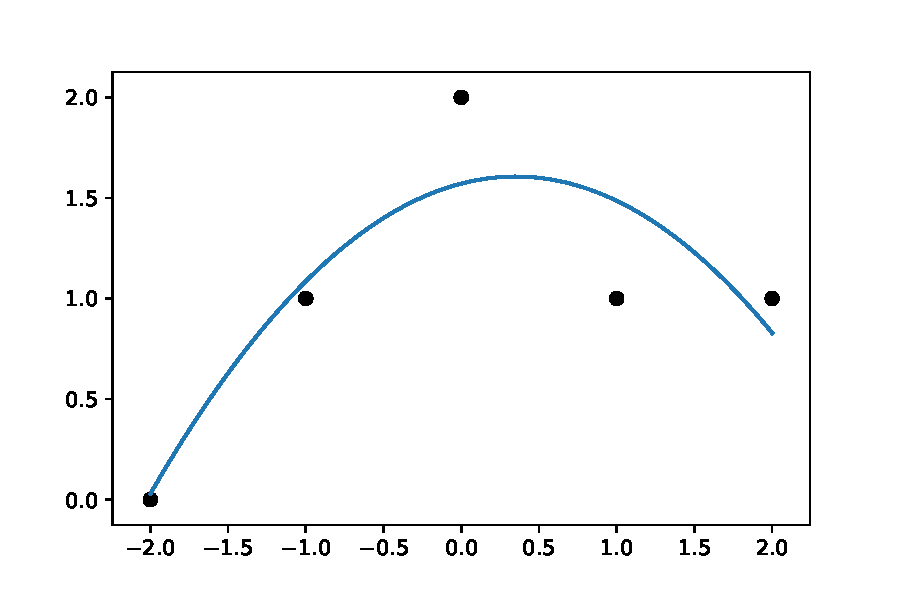
\includegraphics[width=\linewidth]{7-1.pdf}
\end{figure}

设置正则化参数分别为1和10,得到最小二乘解分别如下:
$$f(X)=1.53333333+0.18181818x-0.26666667x^2$$
$$f(X)=\frac{4}{3}+0.1x-\frac{1}{6}x^2$$

将上述三个函数绘图得:

\begin{figure}[H]
	\centering
	\caption{最小二乘及其正则化}
	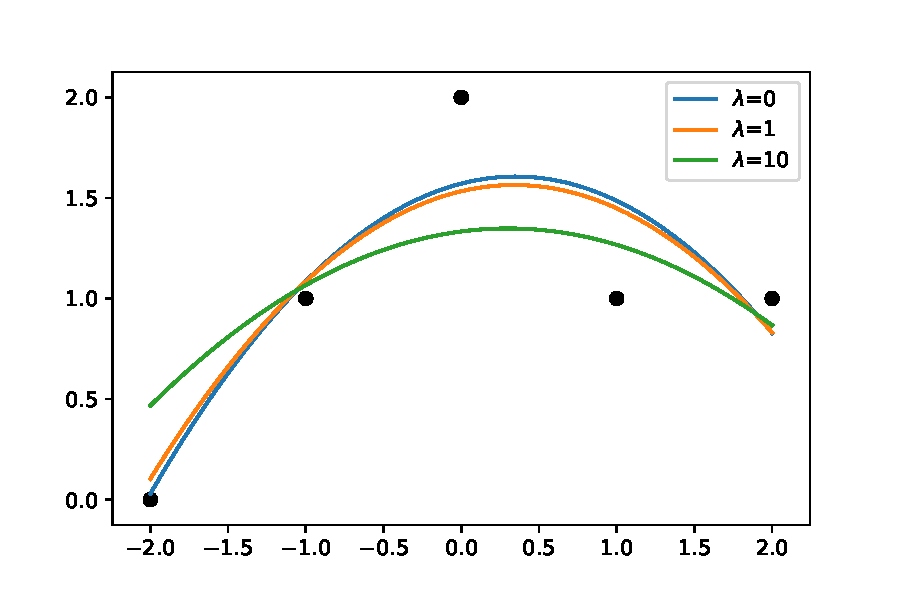
\includegraphics[width=\linewidth]{7-2.pdf}
\end{figure}

\paragraph{代码}

\begin{minted}{python}

lamda=0
I=np.eye(3)
I[0][0]=0
np.linalg.inv(np.matmul(X.T,X)+lamda*I)
theta=np.matmul(np.matmul(np.linalg.inv(np.matmul(X.T,X)+lamda*I),X.T),y)
x0=np.linspace(-2, 2, 100)
m0=len(x0)
x0=x0.reshape([100,1])
x0=np.concatenate((np.ones([100,1]),x0,x0**2), axis=1)
x0=x0.reshape([100,3])

plt.plot(np.linspace(-2, 2, 100),np.matmul(x0,theta),label='$\lambda$=0')
plt.scatter(x,y, color='black')
plt.savefig('7-1.pdf',dpi=200)
plt.show()

lamda=0
I=np.eye(3)
I[0][0]=0
np.linalg.inv(np.matmul(X.T,X)+lamda*I)
theta=np.matmul(np.matmul(np.linalg.inv(np.matmul(X.T,X)+lamda*I),X.T),y)
x0=np.linspace(-2, 2, 100)
m0=len(x0)
x0=x0.reshape([100,1])
x0=np.concatenate((np.ones([100,1]),x0,x0**2), axis=1)
x0=x0.reshape([100,3])
plt.plot(np.linspace(-2, 2, 100),np.matmul(x0,theta),label='$\lambda$=0')
print(theta)

lamda=1
I=np.eye(3)
I[0][0]=0
np.linalg.inv(np.matmul(X.T,X)+lamda*I)
theta=np.matmul(np.matmul(np.linalg.inv(np.matmul(X.T,X)+lamda*I),X.T),y)
x0=np.linspace(-2, 2, 100)
m0=len(x0)
x0=x0.reshape([100,1])
x0=np.concatenate((np.ones([100,1]),x0,x0**2), axis=1)
x0=x0.reshape([100,3])
plt.plot(np.linspace(-2, 2, 100),np.matmul(x0,theta),label='$\lambda$=1')
print(theta)

lamda=10
I=np.eye(3)
I[0][0]=0
theta=np.matmul(np.matmul(np.linalg.inv(np.matmul(X.T,X)+lamda*I),X.T),y)
x0=np.linspace(-2, 2, 100)
m0=len(x0)
x0=x0.reshape([100,1])
x0=np.concatenate((np.ones([100,1]),x0,x0**2), axis=1)
x0=x0.reshape([100,3])
plt.plot(np.linspace(-2, 2, 100),np.matmul(x0,theta),label='$\lambda$=10')
print(theta)



plt.scatter(x,y, color='black')
plt.legend()
plt.savefig('7-2.pdf',dpi=200)
plt.show()


\end{minted}
